% This file was converted to LaTeX by Writer2LaTeX ver. 1.0.2
% see http://writer2latex.sourceforge.net for more info
\documentclass[a4paper]{article}
\usepackage[utf8]{inputenc}
\usepackage[T1]{fontenc}
\usepackage[spanish]{babel}
\usepackage[geometry,weather,misc,clock]{ifsym}
\usepackage{pifont}
\usepackage{eurosym}
\usepackage{amsmath}
\usepackage{wasysym}
\usepackage{amssymb,amsfonts,textcomp}
\usepackage{color}
\usepackage{array}
\usepackage{hhline}
\usepackage{hyperref}
\hypersetup{pdftex, colorlinks=true, linkcolor=blue, citecolor=blue, filecolor=blue, urlcolor=blue, pdftitle=, pdfauthor=Subdirector, pdfsubject=, pdfkeywords=}
\usepackage[pdftex]{graphicx}
% Text styles
\newcommand\textstyleProyectoCursiva[1]{\textit{#1}}
\newcommand\textstyleeacep[1]{#1}
\newcommand\textstyleProyectoNegrita[1]{\textbf{#1}}
% Outline numbering
\setcounter{secnumdepth}{4}
\renewcommand\thesection{\arabic{section}}
\renewcommand\thesubsection{\arabic{section}.\arabic{subsection}}
\renewcommand\thesubsubsection{\arabic{section}.\arabic{subsection}.\arabic{subsubsection}}
\renewcommand\theparagraph{\arabic{section}.\arabic{subsection}.\arabic{subsubsection}.\arabic{paragraph}}
% List styles
\newcommand\liststyleWWviiiNumiii{%
\renewcommand\theenumi{\arabic{enumi}}
\renewcommand\theenumii{\alph{enumii}}
\renewcommand\theenumiii{\roman{enumiii}}
\renewcommand\theenumiv{\arabic{enumiv}}
\renewcommand\labelenumi{[\theenumi]}
\renewcommand\labelenumii{\theenumii.}
\renewcommand\labelenumiii{\theenumiii.}
\renewcommand\labelenumiv{\theenumiv.}
}
% Page layout (geometry)
\setlength\voffset{-1in}
\setlength\hoffset{-1in}
\setlength\topmargin{3cm}
\setlength\oddsidemargin{3cm}
\setlength\textheight{23.352333cm}
\setlength\textwidth{16.5cm}
\setlength\footskip{12.0pt}
\setlength\headheight{12pt}
\setlength\headsep{0cm}
% Footnote rule
\setlength{\skip\footins}{0.119cm}
\renewcommand\footnoterule{\vspace*{-0.018cm}\setlength\leftskip{0pt}\setlength\rightskip{0pt plus 1fil}\noindent\textcolor{black}{\rule{0.25\columnwidth}{0.018cm}}\vspace*{0.101cm}}
% Pages styles
\makeatletter
\newcommand\ps@Convertirxviii{
  \renewcommand\@oddhead{}
  \renewcommand\@evenhead{\@oddhead}
  \renewcommand\@oddfoot{}
  \renewcommand\@evenfoot{\@oddfoot}
  \renewcommand\thepage{\roman{page}}
}
\newcommand\ps@Convertirxvii{
  \renewcommand\@oddhead{}
  \renewcommand\@evenhead{\@oddhead}
  \renewcommand\@oddfoot{}
  \renewcommand\@evenfoot{\@oddfoot}
  \renewcommand\thepage{\roman{page}}
}
\newcommand\ps@Convertirxvi{
  \renewcommand\@oddhead{}
  \renewcommand\@evenhead{\@oddhead}
  \renewcommand\@oddfoot{}
  \renewcommand\@evenfoot{\@oddfoot}
  \renewcommand\thepage{\roman{page}}
}
\newcommand\ps@Convertirxv{
  \renewcommand\@oddhead{}
  \renewcommand\@evenhead{\@oddhead}
  \renewcommand\@oddfoot{}
  \renewcommand\@evenfoot{\@oddfoot}
  \renewcommand\thepage{\roman{page}}
}
\newcommand\ps@Convertirxiv{
  \renewcommand\@oddhead{}
  \renewcommand\@evenhead{\@oddhead}
  \renewcommand\@oddfoot{}
  \renewcommand\@evenfoot{\@oddfoot}
  \renewcommand\thepage{\roman{page}}
}
\newcommand\ps@Convertirxiii{
  \renewcommand\@oddhead{}
  \renewcommand\@evenhead{\@oddhead}
  \renewcommand\@oddfoot{}
  \renewcommand\@evenfoot{\@oddfoot}
  \renewcommand\thepage{\arabic{page}}
}
\newcommand\ps@Convertirxii{
  \renewcommand\@oddhead{}
  \renewcommand\@evenhead{\@oddhead}
  \renewcommand\@oddfoot{}
  \renewcommand\@evenfoot{\@oddfoot}
  \renewcommand\thepage{\arabic{page}}
}
\newcommand\ps@Convertirxi{
  \renewcommand\@oddhead{}
  \renewcommand\@evenhead{\@oddhead}
  \renewcommand\@oddfoot{}
  \renewcommand\@evenfoot{\@oddfoot}
  \renewcommand\thepage{\arabic{page}}
}
\newcommand\ps@Convertirx{
  \renewcommand\@oddhead{}
  \renewcommand\@evenhead{\@oddhead}
  \renewcommand\@oddfoot{}
  \renewcommand\@evenfoot{\@oddfoot}
  \renewcommand\thepage{\arabic{page}}
}
\newcommand\ps@Convertirix{
  \renewcommand\@oddhead{}
  \renewcommand\@evenhead{\@oddhead}
  \renewcommand\@oddfoot{}
  \renewcommand\@evenfoot{\@oddfoot}
  \renewcommand\thepage{\arabic{page}}
}
\newcommand\ps@Convertirviii{
  \renewcommand\@oddhead{}
  \renewcommand\@evenhead{\@oddhead}
  \renewcommand\@oddfoot{}
  \renewcommand\@evenfoot{\@oddfoot}
  \renewcommand\thepage{\arabic{page}}
}
\newcommand\ps@Convertirvii{
  \renewcommand\@oddhead{}
  \renewcommand\@evenhead{\@oddhead}
  \renewcommand\@oddfoot{}
  \renewcommand\@evenfoot{\@oddfoot}
  \renewcommand\thepage{\arabic{page}}
}
\newcommand\ps@Convertirvi{
  \renewcommand\@oddhead{}
  \renewcommand\@evenhead{\@oddhead}
  \renewcommand\@oddfoot{}
  \renewcommand\@evenfoot{\@oddfoot}
  \renewcommand\thepage{\arabic{page}}
}
\newcommand\ps@Convertirv{
  \renewcommand\@oddhead{}
  \renewcommand\@evenhead{\@oddhead}
  \renewcommand\@oddfoot{}
  \renewcommand\@evenfoot{\@oddfoot}
  \renewcommand\thepage{\arabic{page}}
}
\newcommand\ps@Standard{
  \renewcommand\@oddhead{}
  \renewcommand\@evenhead{}
  \renewcommand\@oddfoot{}
  \renewcommand\@evenfoot{}
  \renewcommand\thepage{\arabic{page}}
}
\newcommand\ps@Convertiriv{
  \renewcommand\@oddhead{}
  \renewcommand\@evenhead{\@oddhead}
  \renewcommand\@oddfoot{}
  \renewcommand\@evenfoot{\@oddfoot}
  \renewcommand\thepage{\arabic{page}}
}
\newcommand\ps@Convertiriii{
  \renewcommand\@oddhead{}
  \renewcommand\@evenhead{\@oddhead}
  \renewcommand\@oddfoot{}
  \renewcommand\@evenfoot{\@oddfoot}
  \renewcommand\thepage{\arabic{page}}
}
\newcommand\ps@Convertirii{
  \renewcommand\@oddhead{}
  \renewcommand\@evenhead{\@oddhead}
  \renewcommand\@oddfoot{}
  \renewcommand\@evenfoot{\@oddfoot}
  \renewcommand\thepage{\arabic{page}}
}
\newcommand\ps@Convertiri{
  \renewcommand\@oddhead{}
  \renewcommand\@evenhead{\@oddhead}
  \renewcommand\@oddfoot{}
  \renewcommand\@evenfoot{\@oddfoot}
  \renewcommand\thepage{\roman{page}}
}
\makeatother
\pagestyle{Standard}
\newcounter{Figura}
\renewcommand\theFigura{\arabic{Figura}}
\title{}
\author{Subdirector}
\date{2008-05-06}
\begin{document}
\clearpage\setcounter{page}{1}\pagestyle{Standard}

\bigskip

{\centering\bfseries
UNIVERSIDAD DE ALCALÁ
\par}


\bigskip

{\centering
{\textbf{E}}{\textbf{scuela Técnica Superior de Ingeniería Informática}}
\par}

\begin{figure}
\centering
\includegraphics{TFCPlantilla-img/TFCPlantilla-img1.png}
\end{figure}
{\centering
{\textbf{Ingeniería Informática}}{\textbf{ ó }}
\par}

{\centering\bfseries
Ingeniería Técnica en Informática de XXXXX
\par}


\bigskip

{\centering
Trabajo Fin de Carrera
\par}


\bigskip


\bigskip

{\centering\scshape
Título del tfc
\par}


\bigskip


\bigskip


\bigskip


\bigskip


\bigskip

{\centering\bfseries
Nombre del Autor
\par}

{\centering\bfseries
Año Presentación
\par}

\clearpage
\bigskip

\clearpage
\bigskip

{\centering
UNIVERSIDAD DE ALCALÁ
\par}

{\centering
Escuela Técnica Superior de Ingeniería Informática
\par}

{\centering
{\textsc{Ingeniería Informática}}{\textsc{ ó Lo que proceda}}
\par}


\bigskip

{\centering
Trabajo Fin de Carrera
\par}


\bigskip

{\centering\scshape
TÍTULO DEL TFC
\par}


\bigskip

{
{\textbf{\ \ \ \ Autor}}{\textbf{: \ \ Nombre del autor}}}

{
{\textbf{\ \ \ \ Director: \ \ }}{\textbf{Nombre del director}}}


\bigskip


\bigskip

{
Tribunal:}

{
Presidente: }


\bigskip


\bigskip

{
{Vocal 1º}{: }}


\bigskip


\bigskip

{
Vocal 2º: }


\bigskip

{
{Calificación: }\_\_\_\_\_\_\_\_\_\_\_\_\_\_\_\_\_\_\_\_\_\_\_\_\_\_\_\_\_\_}

{
{Alcalá de Henares a}{ \ \ \ \ \ \ \ de \ \ \ \ \ \ \ \ \ \ \ \ \ \ \ \ \ \ \ \ \ \ \ \ \ \ \ \ \ \ de \ \ \ }}

\clearpage
\bigskip

\clearpage
\bigskip


\bigskip


\bigskip


\bigskip


\bigskip

{
Líneas de agradecimiento, si se quieren poner.}


\bigskip

\clearpage
\bigskip

\clearpage\setcounter{page}{1}\pagestyle{Convertiri}
{\bfseries\scshape
Índice Resumido}


\bigskip

\setcounter{tocdepth}{9}
\renewcommand\contentsname{}
\tableofcontents

\bigskip

\clearpage
\bigskip


\bigskip

\clearpage{\bfseries\scshape
Índice Detallado}


\bigskip
\setcounter{tocdepth}{9}
\renewcommand\contentsname{}
\tableofcontents

\bigskip


\bigskip

\clearpage
\bigskip

{\bfseries\scshape
Índice de Figuras}


\bigskip


\bigskip

{\bfseries\scshape
1.\ \ INTRODUCCIÓN}


\bigskip

{\scshape
{\textbf{2}}{\textbf{.\ \ OBJETIVOS DEL PROYECTO}}}


\bigskip

{\scshape
{\textbf{3}}{\textbf{.\ \ ESTADO DEL ARTE}}}
\listoffigures

\bigskip
\clearpage\setcounter{page}{1}\pagestyle{Convertirii}
{\raggedleft\bfseries\scshape
Introducción
\par}

\clearpage
\bigskip

\clearpage\setcounter{page}{1}\pagestyle{Convertiriii}

\bigskip


\bigskip


\bigskip


\bigskip

{
{\textbf{Introducción en la que se indique el}}{\textbf{ planteamiento del trabajo.}}}


\bigskip

{
{La discapacidad es un hecho tan antiguo como la propia existencia del hombre en la Tierra. La discriminación ha sido la tónica predominante para las personas discapacitadas en todos los aspectos. A lo largo de la historia y especialmente en los últimos años, se han logrado muchos avances en cuanto a accesibilidad. Cada vez son más las facilidades proporcionadas para obtener una calidad de vida equivalente al del resto de personas, pero }{todavía quedan cosas por hacer…}}

\clearpage\setcounter{page}{1}\pagestyle{Convertiriv}
{\raggedleft\bfseries\scshape
Objetivos del Proyecto
\par}

\clearpage
\bigskip

\clearpage\setcounter{page}{1}\pagestyle{Convertirv}

\bigskip


\bigskip


\bigskip


\bigskip

{
{\textbf{Objetivos del Proyecto, donde se exponen}}{\textbf{ los objetivos a conseguir.}}}


\bigskip

{
{Cuando se comenzó a desarrollar software }{de aplicaciones orientadas a usuarios sin ningún tipo de conocimiento específico, su diseño tenía poca consideración hacia éstos: era el usuario el que debía adaptarse al sistema y no al contrario…}}

\clearpage\setcounter{page}{1}\pagestyle{Convertirvi}
{\raggedleft\bfseries\scshape
Estado del Arte
\par}

\clearpage
\bigskip

\clearpage\setcounter{page}{1}\pagestyle{Convertirvii}

\bigskip


\bigskip


\bigskip


\bigskip

{\bfseries
Base teórica en la que se expongan los conceptos teóricos utilizados para la realización del trabajo, así como los cálculos realizados.}


\bigskip

{
{En este }{primer }{capítulo nombrado }\textstyleProyectoCursiva{{Estado del Arte}}{ se pretende ofrecer una base teórica sobre }{cuatro}{ áreas estrechamente relacionadas con el tema central de este escrito: }{la discapacidad y sus tipos, }{la usabilidad y conceptos relacionados, la accesibilidad Web propiamente dicha y las asociaciones y fundaciones que existen en torno a la usabilidad y a la accesibilidad Web…}}


\bigskip

\subsection{Discapacidad}
{
{La Organización Mundial de la Salud, en el año 1980, publicó}{…}}

{
La siguiente clasificación es la que se propone en este trabajo para tener en cuenta:}

{\centering  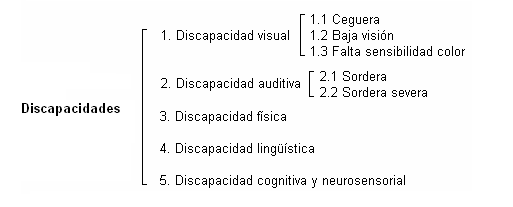
\includegraphics{TFCPlantilla-img/TFCPlantilla-img2.png} \par}

{\centering\bfseries
{Figura }{\stepcounter{Figura}{\theFigura}}{. Clasificación de las discapacidades}
\par}

\subsubsection[Discapacidad visual]{{D}iscapacidad visual}
{
Las deficiencias visuales más comunes…}

\paragraph[Ceguera]{ Ceguera}
{
La ceguera implica…}


\bigskip

\paragraph[Baja visión]{ Baja visión}
{
{Se refiere a aquellas discapacidades que disminuyen la calidad de la visión, sin imposibilitarla}{…}}


\bigskip

\paragraph[Falta de sensibilidad a los colores ]{ Falta de sensibilidad a los colores }
{
{Se traduce en una falta de respuesta a ciertos colores}{…}}


\bigskip


\bigskip

{\centering
 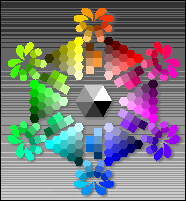
\includegraphics{TFCPlantilla-img/TFCPlantilla-img3.png} { \ \ } 
\includegraphics{TFCPlantilla-img/TFCPlantilla-img4.png} { \ \ } 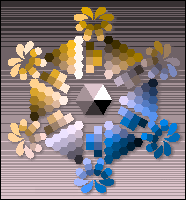
\includegraphics{TFCPlantilla-img/TFCPlantilla-img5.png} { \ \ } 
\includegraphics{TFCPlantilla-img/TFCPlantilla-img6.png} 
\par}

{\centering\bfseries
{Figura }{\stepcounter{Figura}{\theFigura}}{. Paletas de colores según deficiencias visuales}
\par}

{
…}

{\centering   [Warning: Image ignored] % Unhandled or unsupported graphics:
%\includegraphics{TFCPlantilla-img/TFCPlantilla-img7}
 \par}

{
Esos tres botones se verían por una persona con defecto de visión del color de la siguiente manera.}

{\centering   [Warning: Image ignored] % Unhandled or unsupported graphics:
%\includegraphics{TFCPlantilla-img/TFCPlantilla-img8}
   [Warning: Image ignored] % Unhandled or unsupported graphics:
%\includegraphics{TFCPlantilla-img/TFCPlantilla-img9}
   [Warning: Image ignored] % Unhandled or unsupported graphics:
%\includegraphics{TFCPlantilla-img/TFCPlantilla-img10}
 \par}

{
La lección para el diseñador de interfaces es sencilla. No codificar ninguna conducta importante únicamente mediante colores.}


\bigskip


\bigskip

\clearpage\setcounter{page}{1}\pagestyle{Convertirviii}
{\raggedleft\bfseries\scshape
Evaluación de Accesibilidad Web
\par}

\clearpage
\bigskip

\clearpage\setcounter{page}{1}\pagestyle{Convertirix}

\bigskip


\bigskip


\bigskip


\bigskip

{
{\textbf{Descripción experimental, cuando sea necesario, descripción del diseño,}}{\textbf{ resultados, etc.}}}


\bigskip

{
{Este capítulo denominado Evaluación de Accesibilidad }{Web es el más práctico de los vistos hasta ahora debido a que se aplicarán todos los conocimientos teóricos adquiridos para realizar una evaluación exhaustiva de una serie de plataformas Web…}}


\bigskip

\clearpage\setcounter{page}{1}\pagestyle{Convertirx}
{\raggedleft\bfseries\scshape
{Resumen y }{Conclusión}{ }
\par}

\clearpage
\bigskip

\clearpage\setcounter{page}{1}\pagestyle{Convertirxi}

\bigskip


\bigskip


\bigskip


\bigskip

{
{\textbf{R}}{\textbf{esumen }}{\textbf{del trabajo en un máximo de cien (100) palabras. }}}


\bigskip

{
En este último capítulo se realizará un balance de los resultados obtenidos después de la realización del Proyecto Fin de Carrera…}


\bigskip


\bigskip

\subsection{Presupuesto}
{
{\textbf{P}}{\textbf{resupuesto }}{\textbf{(en su caso), que incluya: ejecución material (materiales y mano de obra), gastos generales y beneficio industrial, honorarios de dirección y redacción (tarifas del Colegio, en su caso), coste de ejecución por contrata y presupuesto total.}}}


\bigskip

{
... De esta forma, lo que hacemos es estimar la duración del proyecto en torno a 9 meses con una jornada de 6 horas diarias, exceptuando los fines de semana. Así entonces, obtenemos un total de 1080 horas invertidas en este Proyecto Fin de Carrera…}


\bigskip

\subsection[Conclusiones y Futuras Líneas de Trabajo]{{Conclusiones}{ y Futuras Líneas de Trabajo}}
{\bfseries
Conclusiones y futuro trabajo.}


\bigskip

{
Después de dar por finalizado este Proyecto Fin de Carrera “Accesibilidad en la Web: Normas y Aplicación”, hacemos balance sobre los conocimientos adquiridos y las impresiones obtenidas a lo largo del mismo…}


\bigskip


\bigskip

\clearpage\setcounter{page}{1}\pagestyle{Convertirxii}
{\raggedleft\bfseries\scshape
Bibliografía
\par}

\clearpage
\bigskip

\clearpage\setcounter{page}{1}\pagestyle{Convertirxiii}

\bigskip


\bigskip


\bigskip

{
{\textbf{B}}{\textbf{ibliografía}}{\textbf{, donde se indicará el conjunto de las referencias utilizadas como citas y otros materiales de consulta, siempre que, a lo largo del trabajo, se afirma algo que no se demuestra, conteniendo cada una los siguientes datos:}}}

{\bfseries
{}- Autor/es.}

{\bfseries
{}- Título del artículo, libro, monografía,...}

{\bfseries
{}- Editorial o nombre de la revista y editorial.}

{\bfseries
{}- Número de la revista, volumen y páginas consultadas.}

{\bfseries
{}- Año de publicación.}

{\bfseries
{}- Asimismo, en este apartado se reseñarán los distintos catálogos utilizados.}


\bigskip


\bigskip

\liststyleWWviiiNumiii
\begin{enumerate}
\item {
{Abascal, J., Valero, P. (2001), Curso Introducción a la Interacción Persona-Ordenador: El libro electrónico, AIPO, }\url{http://griho.udl.es/ipo/libroe.html}}
\item {
{Asociación Española de Normalización y Certificación (1986), Normas y Publicaciones }\url{http://www.aenor.es/}{ \ }}
\item {
…}
\end{enumerate}
\clearpage\setcounter{page}{1}\pagestyle{Convertirxiv}
{\raggedleft\bfseries\scshape
Apéndice A. Herramientas de Evaluación y Reparación de Accesibilidad Web
\par}

\clearpage
\bigskip

\clearpage\setcounter{page}{1}\pagestyle{Convertirxv}

\bigskip


\bigskip


\bigskip

{
\textstyleeacep{{\textbf{En un }}}\textstyleeacep{{\textbf{Apéndice s}}}{\textbf{e adjunta información extra, no contenida en puntos anteiores que de más facilidad a la comprensión del tema en cuestión.}}}


\bigskip

{
En este apartado se ofrece una guía de referencia de las herramientas de evaluación y/o reparación de accesibilidad Web existentes en la actualidad…}

\clearpage\setcounter{page}{1}\pagestyle{Convertirxvi}
{\raggedleft\bfseries\scshape
Apéndice B. Glosario
\par}

\clearpage
\bigskip

\clearpage\setcounter{page}{1}\pagestyle{Convertirxvii}

\bigskip


\bigskip


\bigskip


\bigskip

{\bfseries
Un glosario es catálogo de palabras con definición o explicación de cada una de ellas.}


\bigskip

{
{El objetivo de este glosario es facilitar el acceso a una definición de los principales términos que }{se mencionan a lo largo de este libro.}}

{\bfseries
A}

{
\textstyleProyectoNegrita{Accesible. }El contenido es accesible cuando puede ser usado por alguien con discapacidad.}

{
\textstyleProyectoNegrita{{AENOR}}{. }\textstyleProyectoNegrita{{A}}{sociación }\textstyleProyectoNegrita{{E}}{spañola de }\textstyleProyectoNegrita{{NOR}}{malización y }\textstyleProyectoNegrita{{C}}{ertificación, es una entidad dedicada al desarrollo de la normalización y la certificación (N+C) en todos los sectores industriales y de servicios.}}

{
\textstyleProyectoNegrita{{AIPO}}{. }\textstyleProyectoNegrita{{A}}{sociación }\textstyleProyectoNegrita{{I}}{nteracción }\textstyleProyectoNegrita{{P}}{ersona-}\textstyleProyectoNegrita{{O}}{rdenador}}

{
\textstyleProyectoNegrita{{ANSI}}{. }\textstyleProyectoNegrita{{A}}{merican }\textstyleProyectoNegrita{{N}}{ational }\textstyleProyectoNegrita{{S}}{tandards }\textstyleProyectoNegrita{{I}}{nstitute es una organización sin ánimo de lucro que supervisa el desarrollo de estándares para productos, servicios, procesos y sistemas en los Estados Unidos.}}

{
\textstyleProyectoNegrita{{Applet}}{. Componente de software que corre en el contexto de otro programa, por ejemplo un navegador Web.}}

{
\textstyleProyectoNegrita{{ASME}}{. }\textstyleProyectoNegrita{{A}}{merican }\textstyleProyectoNegrita{{S}}{ociety of }\textstyleProyectoNegrita{{M}}{echanical }\textstyleProyectoNegrita{{E}}{ngineers es una asociación profesional, que además ha generado un código de construcción, inspección y pruebas para equipos.}}

{
\textstyleProyectoNegrita{{ASQ}}{. }\textstyleProyectoNegrita{{A}}{merican }\textstyleProyectoNegrita{{S}}{ociety for }\textstyleProyectoNegrita{{Q}}{uality, primeramente conocido como ASQC es una comunidad global basada en el conocimiento formada por expertos de control de calidad. }}

{
\textstyleProyectoNegrita{{ASTM}}{. }\textstyleProyectoNegrita{{A}}{merican }\textstyleProyectoNegrita{{S}}{ociety for }\textstyleProyectoNegrita{{T}}{esting and }\textstyleProyectoNegrita{{M}}{aterials, es una organización de estándares voluntaria internacional que desarrolla y produce estándares técnicos para materiales, productos, sistemas y servicios.}}

{
\textstyleProyectoNegrita{{A}}\textstyleProyectoNegrita{{U}}{. }\textstyleProyectoNegrita{{A}}{gentes de }\textstyleProyectoNegrita{{U}}{suario, es decir, aplicaciones de usuario.}}

{\bfseries
\textstyleProyectoNegrita{{\textmd{B}}}}

{
\textstyleProyectoNegrita{{BITV}}{. }\textstyleProyectoNegrita{{B}}{arrierefreie }\textstyleProyectoNegrita{{I}}{nforma}\textstyleProyectoNegrita{{T}}{ionstechnik }\textstyleProyectoNegrita{{V}}{erordnung. }{Tecnología de la Información Libre de Barreras. Estándar alemán cuyo contenido se basa en las directrices 1.0 de W3C-WAI.}}

{
\textstyleProyectoNegrita{BSI}. \textstyleProyectoNegrita{B}ritish \textstyleProyectoNegrita{S}tandards \textstyleProyectoNegrita{I}nstitution.}

{
...}


\bigskip


\bigskip

\clearpage\clearpage\setcounter{page}{1}\pagestyle{Convertirxviii}

\bigskip


\bigskip
\end{document}
